\documentclass[12pt, openany]{report}
\usepackage[utf8]{inputenc}
\usepackage[T1]{fontenc}
\usepackage[a4paper,left=2cm,right=2cm,top=2cm,bottom=2cm]{geometry}
\usepackage[french]{babel}
\usepackage[pdftex]{graphicx}
\usepackage{float}
\usepackage{hyperref}
\usepackage{listings}
\usepackage[round]{natbib}

\renewcommand{\thesection}{\arabic{section}}

\begin{document}

\author{Colin Baumgard}
\author{Ludovic Diguet}
\author{Hamid Hacene}
\author{Corentin Lemoine}
\author{Antonin Lizé}

\begin{titlepage}
  \begin{sffamily}
    \begin{center}

      \textsc{\LARGE ENSTA Bretagne}\\[2cm]

      \textsc{\Large Projet ROS 4.1}\\[1.5cm]

      % Title
      { \huge \bfseries ROS : implémentation du suivi de ligne sur une voiture à l'échelle 1/10ème\\[0.4cm] }
      \vfill

      \begin{figure}[H]
        \hfill 
\includegraphics[scale=0.6]{img/logoROS.jpg} \hspace*{\fill}
      \end{figure}

      \vfill


      \begin{minipage}{0.30\textwidth}
        Colin \textsc{Baumgard}
      \end{minipage}
      \begin{minipage}{0.30\textwidth}
        Ludovic \textsc{Diguet}
      \end{minipage}
      \begin{minipage}{0.30\textwidth}
        Hamid \textsc{Hacene}
      \end{minipage}
      \begin{minipage}{0.30\textwidth}
        Corentin \textsc{Lemoine}
      \end{minipage}
      \begin{minipage}{0.30\textwidth}
        Antonin \textsc{Lizé}
      \end{minipage}

    \end{center}
  \end{sffamily}
\end{titlepage}

\tableofcontents

\pagebreak

\section{Introduction}
\subsection{Le cahier des charges}

      \begin{figure}[H]
      \begin{center}
        \hfill 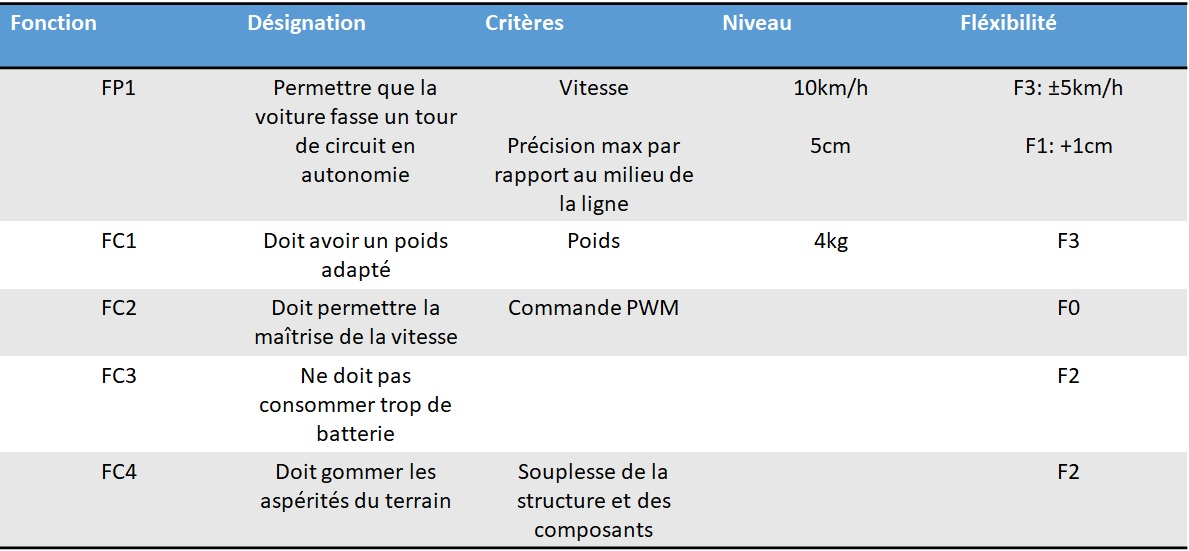
\includegraphics[scale=0.6]{img/Cahier_des_charges.jpg} \hspace*{\fill}
        \caption{Cahier des charges}
      \end{center}
      \end{figure}

      \begin{figure}[H]
      \begin{center}
        \hfill 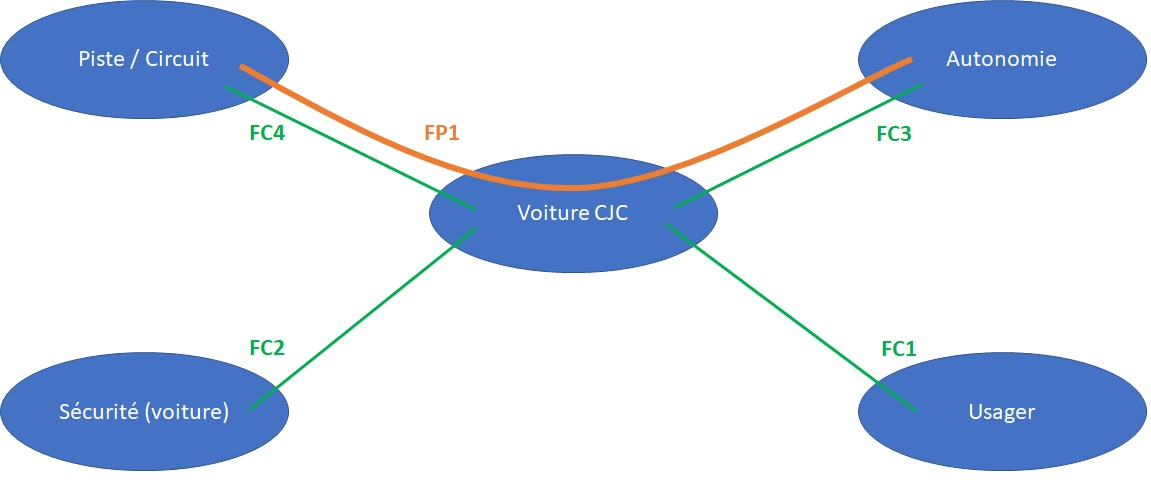
\includegraphics[scale=0.6]{img/Diagramme_pieuvre.jpg} \hspace*{\fill}
        \caption{Diagramme pieuvre}
      \end{center}
      \end{figure}

      \begin{figure}[H]
      \begin{center}
        \hfill 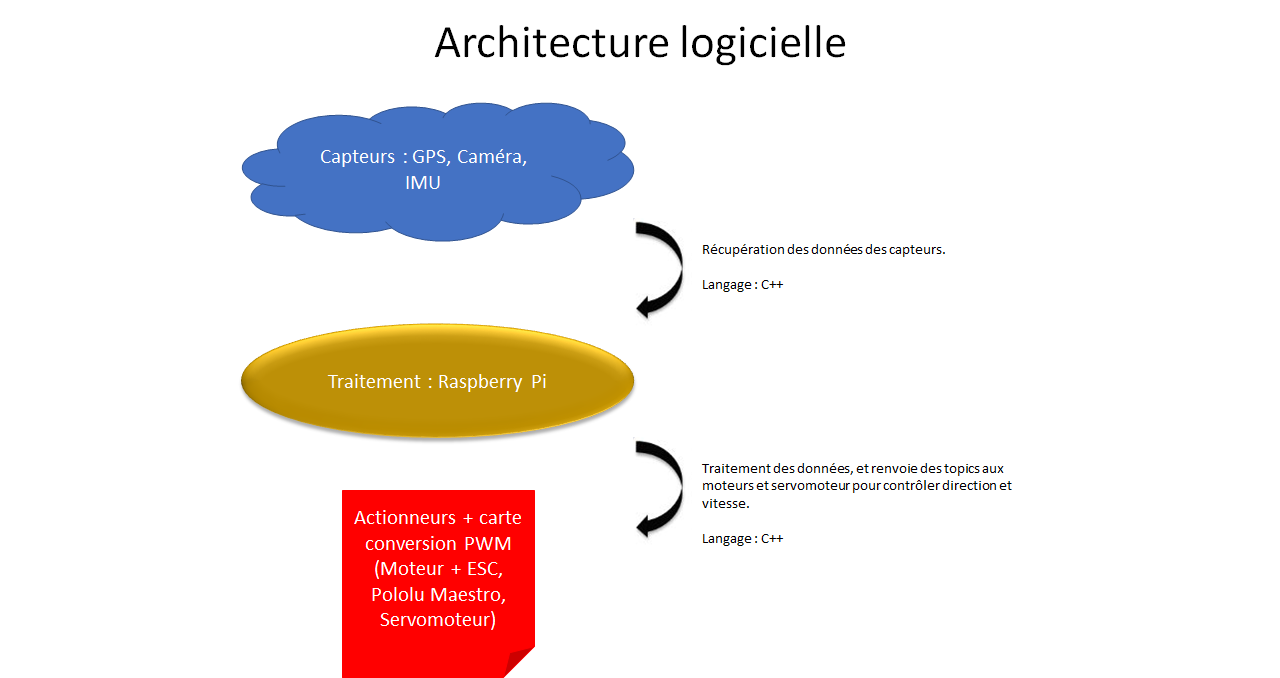
\includegraphics[scale=0.6]{img/Architecture_Logicielle_Materielle.png} \hspace*{\fill}
        \caption{Architecture Logicielle Matérielle}
      \end{center}
      \end{figure}


\subsection{Les pistes envisagées}
Lorem ipsum dolor sit amet

\section{Structure du projet}
\subsection{Lancement du programme}
Lorem ipsum dolor sit amet

\begin{lstlisting}
          roslaunch waypoints_follow seeMeRollin.launch
    \end{lstlisting}

\subsection{Packages}
\subsubsection{Drivers}
Les drivers sont implémentés en utilisant le plus possible les nodes distribuées avec ROS. Le driver du GPS est celui du package \emph{nmea\_navsat\_driver} ;
la node utilisée est \emph{nmea\_serial\_driver}. La node \emph{navsat\_transform\_node} du package \emph{robot\_localization} transforme alors la donnée
issue du driver en une projection dans le repère du robot.

Le package \emph{cv\_camera} nous permet de publier une image sur un topic ROS issue de la caméra de la Raspberry pi.

Pour l'envoi de signaux $PWM$ vers l'ESC et le servo de direction, on a codé une node Python utilisant une bibliothèque pour contrôler la carte Maestro via
la connexion série USB.


\subsubsection{Traitement d'image}
Lorem ipsum dolor sit amet

\subsubsection{Contrôleur}
Lorem ipsum dolor sit amet

Exemple latex langage c :
\begin{lstlisting}[language=C]
        __kernel void mandelbrot(__global float2 *q, 
        __global ushort *output, ushort const maxiter)
        {
            int gid = get_global_id(0);
            float nreal, real = 0;
            float imag = 0;
            output[gid] = 0;
            for(int curiter = 0; curiter < maxiter; curiter++) {
                nreal = real*real - imag*imag + q[gid].x;
                imag = 2* real*imag + q[gid].y;
                real = nreal;
                if (real*real + imag*imag > 4.0f)
                    output[gid] = curiter;
            }
        }
      \end{lstlisting}

\section{Conclusion}
Lorem ipsum dolor sit amet


\bibliographystyle{unsrtnat}
\bibliography{my_bibtex}
\end{document}